\section{Motors}
This section will propose two different types of motors the robot could use in the solution proposal.

\subsection{AC motor}
An AC generator use the principal Faraday‘s electromagnetic induction to convent a mechanical energy such a rotation, into electrical energy. Faraday‘s law of induction – the physical phenomenon when the electric current starts to flow through a conductor in a variable magnetic field or in a moving constant magnetic field. \\

\begin{figure}[h]
    \centering
    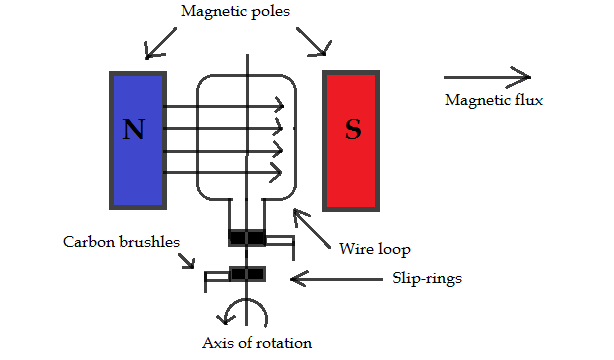
\includegraphics[width=.7\textwidth]{figures/Alternative_current_(AC).png}
    \caption{Alternative current motor } 
    \label{fig:ACmotor} 
\end{figure}

AC motor consist of see at he figure\ref{fig:ACmotor} : Wire loop- rotated ground a fixed axis allowing it to at the magnetic flux at various angles.
Slip-rings-used to transfer the electrical current induced in the coil.
Carbon brushes-make continuous contact between the external circuit and the slip rings.
Rotor-rotating part.
Stator-not moving part.\\
As the coil rotates anticlockwise around the central axis which is perpendicular to the magnetic field, the wire loop cuts the lines of magnetic force set up between the north and south poles at different angles as the loop rotates.
The amount of electro-motive force induced into a coil cutting the magnetic lines at force is determined by the following thee factors:\\
Speed - the speed at which the coil rotates inside the magnetic field.\\
Strength -the strength of the magnetic field.\\
Length - the length of the coil or conductor passing through the magnetic field.\\

\begin{figure}[h]
    \centering
    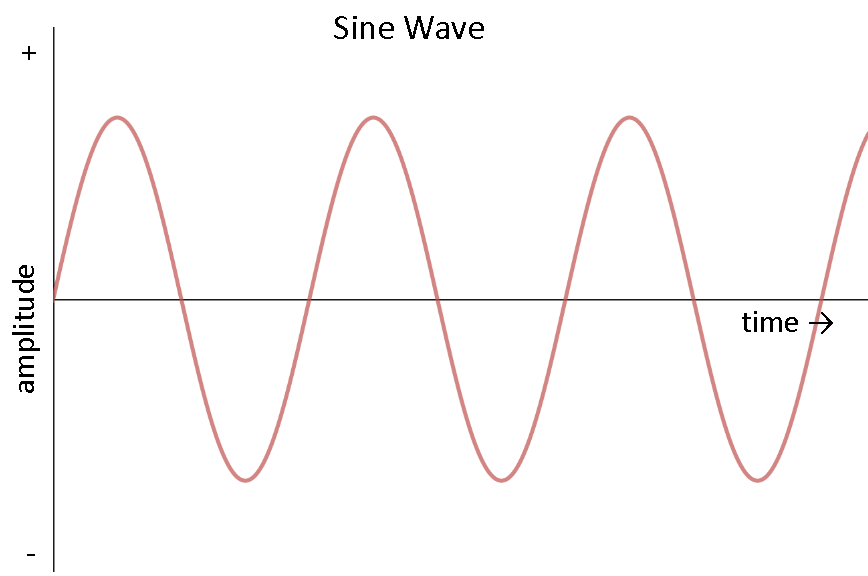
\includegraphics[width=.7\textwidth]{figures/wave.png}
    \caption{Sine wave of AC motor \cite{ACmotor3}} 
    \label{fig:ACmotor1} 
\end{figure}

Sinusoid is used to describe any waveform that has the same shape. The line graph shows how shifted the waveform is with respect to time, see figure \ref{fig:ACmotor1}. Periodic nature of the sine wave, if the wave form is shifted by 360° it becomes the same waveform again, as if it was shifted by 0°. 

\subsection{DC motor}
 Direct current motors provides constant voltage or current. A simple DC generator consists of the same basic elements as a simple AC generator, such as magnetic poles, carbon brushes, wire coil, see figure \ref{fig:DCmotor}. The main difference between a DC motor and an AC motor lies in the manner in which the rotating coil is connected to the external circuit containing the load. Furthermore, in DC motors  are using commutator instead of slip rings, with ones excess the same function like slip rings. 
 
 \begin{figure}[h]
    \centering
    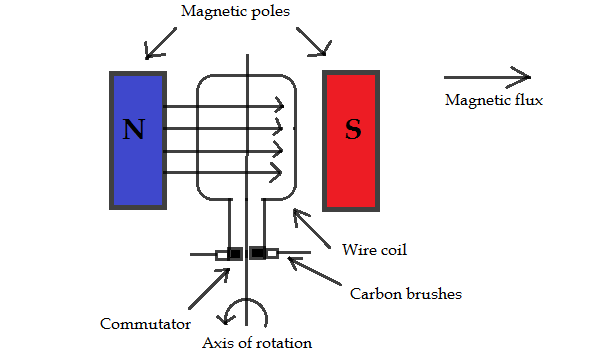
\includegraphics[width=.7\textwidth]{figures/Directcurrent(DC).png}
    \caption{Direct current motor } 
    \label{fig:DCmotor} 
\end{figure}

Moreover, in a DC generator, the two ends of the coil are attached to different halves of commutator which co-rotates with the coil.

 \begin{figure}[h]
    \centering    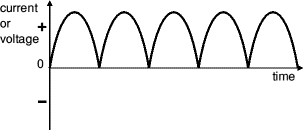
\includegraphics[width=.7\textwidth]{figures/graphDC.png}
    \caption{Working graph of DC motor } 
    \label{fig:DCmotor1} 
\end{figure}

The output of the DC motor is shown in figure \ref{fig:DCmotor1}. The output is not steady but is always in the same direction. As with the AC motor the maximum output voltage occurs when the coil is horizontal and is cutting the field at right angles and at maximum rate.
%\newpage

%conclusion  - put them up against each other